\Chapter{Tervezés}
\Section{Nyelv használat}
A program HTML, JavaScript nyelven fog íródni, canvas használatával. Illetve az objektum orientált programozáshoz igazodva osztályokat fog használni. Ezekből 3 darabra lesz szükség. 


\Section{Megjelenítés kezdetek} 


A program kezdetében először el kell dönteni, hogy hogyan rajzoljuk ki a köröket. Ehhez 2 módszer is szóba jöhet. Aztán ezek közül ki kell választani, nyilván azt amelyik gyorsabbnak bizonyul. 

\Section{Mozgatás}

Ha kész a megjelenítés, akkor jöhet a mozgatás. Aminél számításba kell venni, hogy a gravitációnak kell a körökre hatnia. 

\Section{Ütközések}

Ha megvan a mozgás utána jöhet az ütközések vizsgálata, aminél érdemes először a falakkal kezdeni. Aztán ha az megvan jöhet a körök egymás közötti ütközése is. 

\Section{Akadályok}

Aztán ha az ütközések is megvannak jöhetnek az akadályok, ami nekünk valószínűleg egy pohár lesz. Aztán erre/ezekre az akadályokra is szükséges megírni az ütközésvizsgálatokat. 


\Section{UML}
Ha megvagyunk a program tervezésével jöhet az UML diagram. A következő ábrán \Aref{fig:dia} a programhoz kapcsolódó UML diagram látható. Jól látható a 3 osztály és a közöttük lévő kapcsolatok, illetve a bennük lévő attribútumok és műveletek. 


\begin{figure}[h]
	\centering
	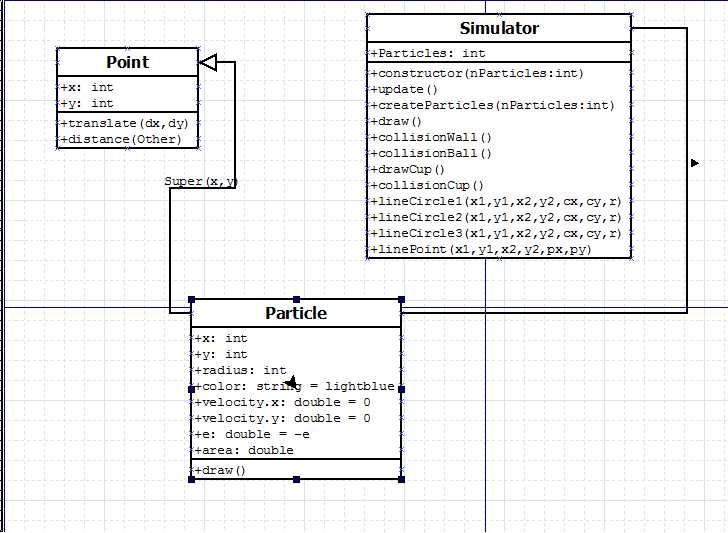
\includegraphics[scale=1]{images/dia.png}
	\caption{UML diagram}
	\label{fig:dia}
\end{figure}


Jól látható, hogy a Particle osztály, a Point osztály leszármazottja, 2 származtatott metódussal.

Mindegyik osztály tartalmaz attribútumokat és műveleteket is. 

